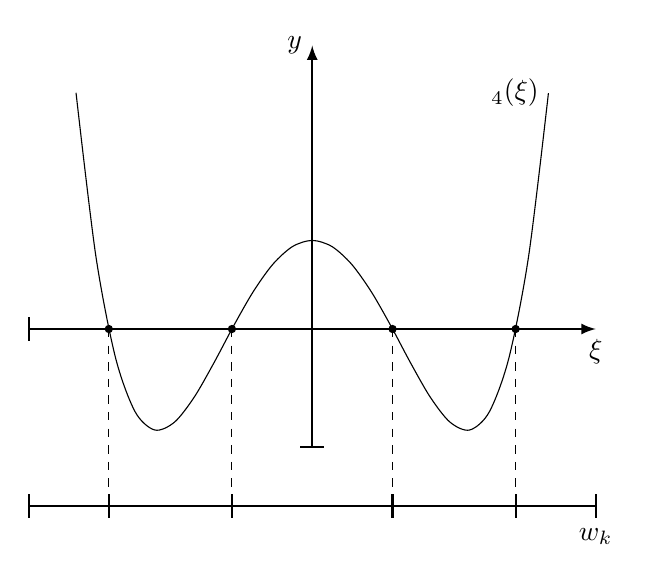
\begin{tikzpicture}
  \begin{scope}[scale = 3]
    \def\xmax{1.2}
    \def\ymin{-.5}
    \draw[-latex, thick] (-\xmax, 0)--(\xmax, 0) node[below]{$\xi$};
    \draw[thick] (-\xmax, .05)--(-\xmax, -.05);
    \draw[-latex, thick] (0, -.5)--(0, \xmax) node[left]{$y$};
    \draw[thick] (-.05, \ymin)--(.05, \ymin);
    \draw[domain = -1:1] plot[smooth] (\x, {4.375*(\x)^4 - 3.75*(\x)^2 + .375}) node[left]{$\legendre_4(\xi)$};
    \def\weightline{-.75}
    \draw[thick] (-\xmax, \weightline)--(\xmax, \weightline) node[below = 1ex]{$w_k$};
    \draw[thick] (-\xmax, {\weightline + .05})--(-\xmax, {\weightline - .05});
    \draw[thick] (\xmax, {\weightline + .05})--(\xmax, {\weightline - .05});
    \foreach \k in {1,2} {
      \foreach \x in {0.861136, 0.339981} {
        \def\xcoord{{(-1)^(\k) * \x}}
        \draw[fill = black] (\xcoord, 0) circle (.015);
        \draw[dashed] (\xcoord, 0) -- (\xcoord, \weightline);
        \ifthenelse{\equal{\x}{0.861136}}{%
          \def\fraction{$\frac{18-\sqrt{30}}{36}$}
        }{%
          \def\fraction{$\frac{18+\sqrt{30}}{36}$}
        }
        \draw[thick] (\xcoord, {\weightline + 0.05})--(\xcoord, {\weightline - 0.05}) node[below]{\fraction};
      }
    }
  \end{scope}
\end{tikzpicture}
